\documentclass[conference]{IEEEtran}
\IEEEoverridecommandlockouts
\usepackage{cite}
\usepackage{amsmath,amssymb,amsfonts}
\usepackage{algorithmic}
\usepackage{graphicx}
\usepackage{textcomp}
\usepackage{xcolor}
\usepackage{booktabs}
\usepackage{array}
\usepackage{hyperref}
\usepackage{url}
\usepackage{float}
\usepackage{subcaption}

\graphicspath{{figs/}}

\begin{document}

\title{The Forward-Fill Lag Trap: Target Leakage in Sparse Event Time Series and a Stop-Level Fix for Transit Demand Classification}

\author{
  \IEEEauthorblockN{Vignan Kamarthi\IEEEauthorrefmark{1} and Aadit Bhatia\IEEEauthorrefmark{2}}
  \IEEEauthorblockA{
    \IEEEauthorrefmark{1}Khoury College of Computer Sciences,
    Northeastern University, Boston, MA 02115, USA\\
    \IEEEauthorrefmark{2}College of Science,
    Northeastern University, Boston, MA 02115, USA\\
    Email: \{kamarthi.v, bhatia.aa\}@northeastern.edu
  }
}

\maketitle

\begin{abstract}
Urban transit operators need stop-level short-term demand forecasts to
dispatch vehicles, adjust schedules, and allocate drivers in real time.
We study 3-class (low/medium/high) ridership demand classification on
the ZTBus dataset (1,409 trolleybus missions, Zurich 2019--2022) under
mission-level temporal splits (pre-2022 train, 2022 test) that mirror
realistic deployment. Our best model, a Random Forest with stop-level
lag features, reaches temporal macro-F1 = 0.8287 ($+0.2221$ over a
57-feature cross-sectional baseline of GPS, speed, power, and calendar
features). Along the way we identify and fix a subtle target-leakage
pattern that arises when standard 1~Hz lag features are computed on
forward-filled sparse passenger counts: the naive lag becomes a
near-exact copy of the current value for roughly 95\% of rows.
Computing lag features at the natural stop-event granularity, then
forward-filling the lag values, eliminates the leakage while
preserving the autoregressive signal. We additionally report a
negative result: adding TimesFM~2.5-200M penultimate-layer embeddings
(1280-dim, PCA-reduced to 32) on top of stop-level lags does not
improve any model (F1 = 0.8241, a change of $-0.005$ relative to
stop-lags-only under a single fixed training seed). The 32 retained
components capture 100\% of the training-embedding variance,
suggesting the foundation model's bus-ridership representations
collapse onto a low-rank subspace already spanned by recent-stop
history. Our contributions are (i) a strong applied result for
stop-level transit demand classification, (ii) a diagnosis and
practical fix for the forward-fill lag trap as a general
practitioner's caution, and (iii) a null result on zero-shot
foundation-model feature extraction for structured event data.
\end{abstract}


\begingroup
\renewcommand\thefootnote{}\footnotetext{\textbf{Code and data availability.}
All code, preprocessing scripts, model training pipelines, results, and
figures are openly available at
\url{https://github.com/vignankamarthi/Scalable-Demand-Optimization-}.
The ZTBus dataset is publicly available via the ETH Research Collection
at \url{https://doi.org/10.3929/ethz-b-000626668} under CC-BY-4.0.}
\addtocounter{footnote}{-1}
\endgroup

\begin{IEEEkeywords}
time series classification, feature engineering, target leakage, foundation models, transit demand, urban mobility, random forest, TimesFM
\end{IEEEkeywords}

\section{Introduction}
\label{sec:intro}

Urban bus systems are the backbone of public transit in many cities. Fleet
operators need near-real-time estimates of which stops and corridors will see
the highest passenger volumes so they can dispatch additional vehicles,
adjust schedules, and allocate drivers. Historically this has been done with
aggregated historical averages and manual reporting, but the availability of
instrumented vehicles (buses with GPS, powertrain sensors, and on-board
passenger counters) has opened the door to data-driven forecasting with
graph and attention models for stop-level demand \cite{li2023pagtsn}.

Modern transit sensor data exhibits a characteristic structural pattern:
dense continuous telemetry (GPS at 1~Hz, speed, power, braking force) arrives
alongside sparse event data (passenger counts updated only when doors open
at stops, typically every 60--120 seconds of driving time). The sparse
series covers approximately 1\% of rows in a raw 1~Hz stream, with the vast
majority of rows carrying only implicit ``no change'' information. This mix
of dense-and-sparse is common in IoT and mobility applications more broadly.

Data scientists approaching this kind of data default to two well-known
preprocessing steps. First, they forward-fill the sparse series onto the
dense timeline, justified by the physical argument that passenger count is
constant between stops (no one boards or alights while the bus is moving).
This transforms 0.9\% usable data into approximately 99\%. Second, they
compute lag features on the now-dense series to capture temporal context,
for example, \texttt{lag(60\,s)} and \texttt{lag(300\,s)} to match typical
rolling-window sizes.

\textbf{An obstacle.} Standard 1~Hz lag features computed on the
forward-filled passenger count series induce target leakage: forward-fill
makes the series piecewise constant between stop events (roughly every
60--120 seconds), and typical lag windows (60~s, 300~s) rarely cross a
stop boundary, so \texttt{lag(60\,s)} equals the current value for
approximately 95\% of rows. Section~\ref{sec:methods-v1} diagnoses the
mechanism in detail; Section~\ref{sec:methods-v2} presents the fix:
compute lag features at stop-event granularity, then forward-fill the
lag values onto the dense grid rather than forward-filling the raw
series first.

\textbf{Baseline.} Our reference point is a standard tree-model pipeline
(Decision Tree, Random Forest, XGBoost) trained on 53 handcrafted sensor
and temporal features (GPS, speed, power, acceleration, time-of-day,
day-of-week, weather) with no passenger count information. On temporal
splits this baseline reaches macro-F1 0.57 for Decision Tree and 0.6066
for Random Forest. The contributions below are measured against these
numbers.

\textbf{Our contributions.}
\begin{enumerate}
  \item We present a strong applied result for stop-level transit demand
    classification on the ZTBus dataset~\cite{widmer2023ztbus}, a
    1,409-mission trolleybus dataset from Zurich, 2019--2022: a Random
    Forest with stop-level lag features reaches temporal macro-F1 =
    0.8287 ($+0.2221$ over the 57-feature cross-sectional baseline) on
    the realistic pre-2022 train, 2022 test evaluation.
  \item We document and fix the forward-fill lag trap underlying this
    result. Adding naively computed 1~Hz passenger-count lag features on
    forward-filled data lifts the Decision Tree from macro-F1 0.57 to
    0.87, but we show this 30-point jump is target leakage: for
    60-second lags on 1~Hz data, approximately 95\% of rows satisfy
    \texttt{lag(60\,s) = current}, so the lag feature is a near-copy of
    the target. Our fix computes lag features at the natural event
    granularity (stop events) and then forward-fills the \emph{lag
    values} onto the dense grid. The resulting features carry genuine
    autoregressive information because they come from strictly earlier
    stops.
  \item We present a negative result on foundation-model feature
    extraction. TimesFM~2.5-200M~\cite{das2024timesfm} penultimate-layer
    embeddings (1280-dim, PCA-reduced to 32) do not improve any model
    beyond the hand-crafted stop-level lags. PCA explained variance
    reaches 100\% at 32 components, indicating the foundation model's
    representations for this domain live in a low-rank subspace. We
    interpret this as the embeddings being largely redundant with
    recent-stop history.
  \item We release a reproducible pipeline implementing all of the
    above, including the event-marker design that enables stop-level
    feature computation through a forward-fill-based preprocessing
    pipeline.
\end{enumerate}

\textbf{Roadmap.} Section~\ref{sec:related} surveys related work.
Section~\ref{sec:data} describes the ZTBus dataset and the classification
task. Section~\ref{sec:eda} presents exploratory analysis.
Section~\ref{sec:methods} develops the methodology, including the leakage
diagnosis and fix. Section~\ref{sec:results} reports quantitative results.
Section~\ref{sec:discussion} discusses generalization and limitations, and
Section~\ref{sec:conclusion} concludes.

\section{Related Work}
\label{sec:related}

\subsection{Transit demand forecasting}

Short-term transit demand prediction has been studied extensively. Classical
approaches rely on time series regression or ARIMA on aggregated ridership
data \cite{box1976timeseries}. More recently, graph neural networks have
been used to model spatial dependencies between stops: Li et
al.~\cite{li2023pagtsn} propose PAG-TSN, a parallel attention graph network
for ridership demand that exploits inter-stop adjacency in smart
transportation services. Tree-ensemble baselines (Random Forest, gradient
boosting) remain competitive on tabular transit features, particularly
when combined with classical temporal predictors such as lag terms and
rolling statistics. The ZTBus dataset we use was introduced by Widmer et
al.~\cite{widmer2023ztbus}, which describes the collection protocol and
channel schema but does not present a demand classification pipeline.

\subsection{Time series foundation models}

A recent generation of large pretrained models aims to provide universal
time series forecasting capabilities analogous to language models for text.
TimesFM~\cite{das2024timesfm}, a 200M-parameter decoder-only transformer
from Google Research, and related models such as Chronos, Moirai, and
Lag-Llama follow similar patterns: patch the time series, embed via a
tokenizer, pass through a stack of transformer layers, and project to a
forecast head. Empirical evaluation of these models remains an open
research area: Meyer et al.~\cite{meyer2025benchmarking} survey
benchmarking challenges specific to time series foundation models,
highlighting risks of information leakage through overlapping datasets
and the memorization of global patterns from external shocks. Our work
uses TimesFM not as a forecaster but as a \emph{feature extractor}, a use
case that has received less empirical scrutiny and, as we show, exposes
limitations in the generality of its learned representations when applied
to structured tabular downstream tasks.

\subsection{Feature leakage and evaluation integrity}

Feature leakage, the accidental introduction of target information into
features, is a long-recognized pitfall in applied machine
learning~\cite{kaufman2012leakage}. Kaufman et al.\ formalize leakage as
the inclusion of data in the training process that would not legitimately
be available at prediction time, enumerate common sources (time-based
leakage, target encoding, group-based splits), and recommend a set of
detection and avoidance strategies. In time series contexts specifically,
leakage can arise from train-test temporal overlap, look-ahead bias in
rolling statistics, or cross-series correlation at the benchmark
level~\cite{meyer2025benchmarking}. Our contribution identifies a
different class of leakage: not at evaluation time, but at \emph{feature
engineering} time, introduced by an interaction between imputation and
feature computation that appears benign when the two steps are examined
separately.

\subsection{Sparse event time series}

Sparse event data is common in many domains: medical vital signs recorded
only during checkups, IoT sensor readings that trigger on thresholds, and
financial tick data between quotes. Bagattini et
al.~\cite{bagattini2019sparse} propose a classification framework
specifically for sparse multivariate temporal features in medical records,
introducing a three-phase symbolic transformation that handles variable
sparsity without imputation. Dillmann et al.~\cite{dillmann2024events}
develop sparse autoencoder representations of event time series for
high-energy astrophysics, operating directly on energy-time binned event
files without intermediate regularization. Che et
al.~\cite{che2018grud} introduce GRU-D, which directly models
missing-value patterns in multivariate healthcare time series rather than
imputing at all. All of these approaches address sparsity by building
models that treat sparsity as a first-class signal. We take the opposite
approach: we use forward-fill imputation for its simplicity and physical
grounding, then fix the resulting leakage at the feature engineering
stage rather than the model.

\subsection{Classical time series analysis}

Our work makes extensive use of classical time series tools. Box and
Jenkins~\cite{box1976timeseries} provide the foundational ARIMA framework
we use for our temporal-only baseline. Dickey and
Fuller~\cite{dickey1979unit} and Kwiatkowski et
al.~\cite{kwiatkowski1992kpss} provide the ADF and KPSS unit root tests,
which we apply in complementary fashion to establish stationarity
properties. Autocorrelation (ACF) and partial autocorrelation (PACF)
diagnostics remain the standard tools for characterizing temporal memory
in a series.

\section{Data and Problem Setup}
\label{sec:data}

\subsection{The ZTBus dataset}

We use the ZTBus dataset introduced by Widmer et
al.~\cite{widmer2023ztbus}, released under CC-BY-4.0. The dataset contains
1,409 trolleybus missions recorded by two HESS lighTram~19 DC articulated
vehicles operated by Verkehrsbetriebe Z\"urich (VBZ) in Zurich,
Switzerland, between April 2019 and December 2022. Each mission is one
complete driving assignment (from pull-out to pull-in) of typically 3--10
hours' duration. Sensor data is recorded at 1~Hz across 26 channels
covering GPS, odometry, electric powertrain, temperature, door state, and
passenger count reported by the on-board Integrated Traffic Control System
(ITCS).

Each mission CSV contains 1~Hz sensor data with timestamps in both ISO and
Unix formats. A separate metadata file lists mission-level attributes:
start/end times, bus number, bus route, and driven distance. The dataset
covers 10 bus routes, with Route~83 accounting for approximately 60\% of
all missions. We use all 1,409 missions in our experiments.

\subsection{The sparse event pattern}

The \texttt{itcs\_numberOfPassengers} channel, the source of our target
variable, is sparse. The ITCS updates passenger count only at stop events,
when doors open and passengers board or alight. At the 1~Hz sampling rate,
only approximately 1\% of rows contain a genuine passenger count; the
remainder are \texttt{NaN}. Stop events occur roughly every 60--120 seconds
of driving time, with some variability depending on route characteristics
(dwell time, stop spacing, time of day).

We forward-fill \texttt{itcs\_numberOfPassengers} within each mission: rows
between stop events inherit the most recent known passenger count. This is
physically justified: passenger count cannot change while the bus is in
motion between stops, and it transforms the 0.9\% usable rows into
approximately 99\% (rows before the first stop of a mission remain
\texttt{NaN} and are dropped). After forward-fill and dropping pre-first-stop
rows, we have 47,628,626 usable rows across the 1,409 missions.

Critically, we preserve the original \texttt{NaN} pattern as a boolean
column \texttt{is\_stop\_event}. A row is a stop event if and only if its
\texttt{itcs\_numberOfPassengers} was non-\texttt{NaN} before forward-fill.
This marker is what enables the stop-level lag feature computation
described in Section~\ref{sec:methods}. Figure~\ref{fig:leakage} illustrates
the forward-fill staircase and the role of \texttt{is\_stop\_event}.

\subsection{Classification task and target construction}

We formulate the problem as 3-class ridership demand classification at
stop-time granularity. For each row in the dense (forward-filled) stream,
we predict whether the current passenger count is \emph{low}, \emph{medium},
or \emph{high}. The class boundaries are tercile thresholds $(q_1, q_2)$
computed from the training partition of \texttt{itcs\_numberOfPassengers}:
\begin{equation}
y(t) = \begin{cases}
  \text{low}    & \text{if } p(t) \le q_1 \\
  \text{medium} & \text{if } q_1 < p(t) \le q_2 \\
  \text{high}   & \text{if } p(t) > q_2
\end{cases}
\end{equation}
where $p(t)$ is the passenger count at row $t$. On the full dataset,
$q_1 \approx 9$ and $q_2 \approx 19$ passengers. The resulting class
distribution is approximately balanced at 37\% low, 32\% medium, 32\% high
(Figure~\ref{fig:passenger-dist}). Importantly, the tercile boundaries are
computed \emph{exclusively} on the training data to prevent test-set
information from leaking into the target definition.

\begin{figure}[t]
  \centering
  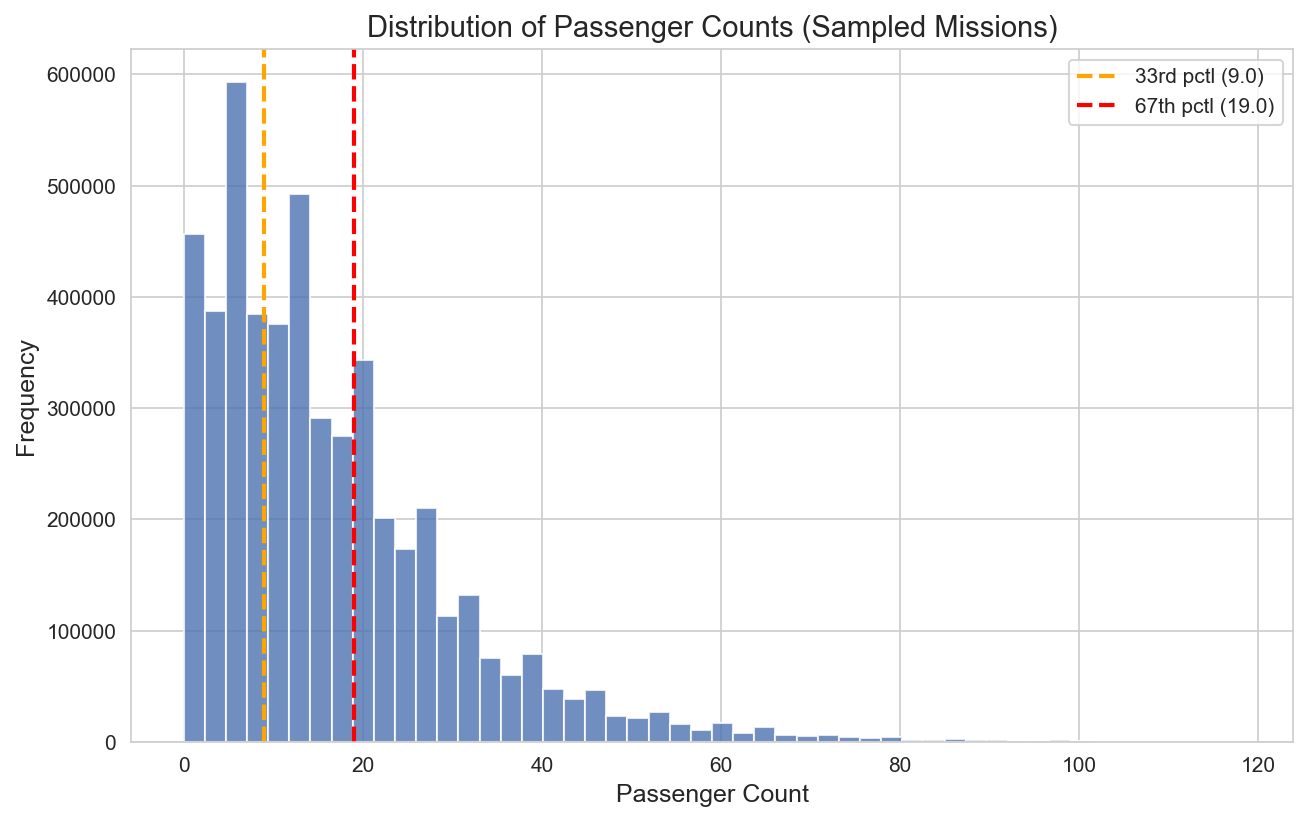
\includegraphics[width=\columnwidth]{01_passenger_distribution.png}
  \caption{Distribution of passenger counts across all ZTBus stop events,
    with tercile boundaries $q_1 \approx 9$ and $q_2 \approx 19$ marked.
    The resulting 3-class target is approximately balanced (37/32/32\%).}
  \label{fig:passenger-dist}
\end{figure}

\subsection{Evaluation frameworks}

We evaluate under two splitting strategies:
\begin{itemize}
  \item \textbf{Pooled split.} 80/20 mission-level random split. Train and
    test come from the same distribution. This measures in-distribution
    generalization.
  \item \textbf{Temporal split.} Missions starting before 2022-01-01 are
    training (811 missions, 57.6\%, covering April 2019 through
    December 2021); missions starting in 2022 are test (598 missions,
    42.4\%, covering January through December 2022). The 57/42
    proportion is closer to balanced than a conventional 80/20 temporal
    cut because 2022 was the single most data-rich year in the dataset
    (598 missions, compared to 147 in 2019, 174 in 2020, and 490 in
    2021). This measures generalization to future data and is the more
    realistic deployment scenario.
\end{itemize}

We report macro-averaged F1 score and balanced accuracy under both
frameworks, plus $3\times 3$ confusion matrices and per-class
precision/recall. Macro-F1 is our primary metric because it weights classes
equally, preventing the majority class from dominating the evaluation under
any class imbalance.

\subsection{Mission-level splits prevent row-level leakage}

All splits are at the mission level, not the row level. Since a single
mission generates tens of thousands of 1~Hz rows, a row-level random split
would scatter the same mission across train and test, giving the model
indirect access to other rows from the same trip (highly correlated
neighbors via rolling features, nearby stops, and shared contextual
features). Mission-level splits ensure that a mission is entirely in one
partition.

\section{Exploratory Data Analysis}
\label{sec:eda}

Before building models, we characterized the data through a suite of
exploratory visualizations. Five findings shaped the feature engineering
decisions of Section~\ref{sec:methods}.

\textbf{Finding 1: Ridership follows strong daily and weekly cycles.}
Figure~\ref{fig:hour} shows mean passenger count by hour of day, separated
by weekday and weekend. Weekdays exhibit pronounced morning (7--9~AM) and
afternoon (4--7~PM) peaks typical of commuter transit, while weekends show
a broader single midday peak centered around 1--3~PM. This justifies
including \texttt{hour}, \texttt{dayofweek}, and \texttt{is\_rush\_hour}
as calendar-derived temporal features.

\begin{figure}[t]
  \centering
  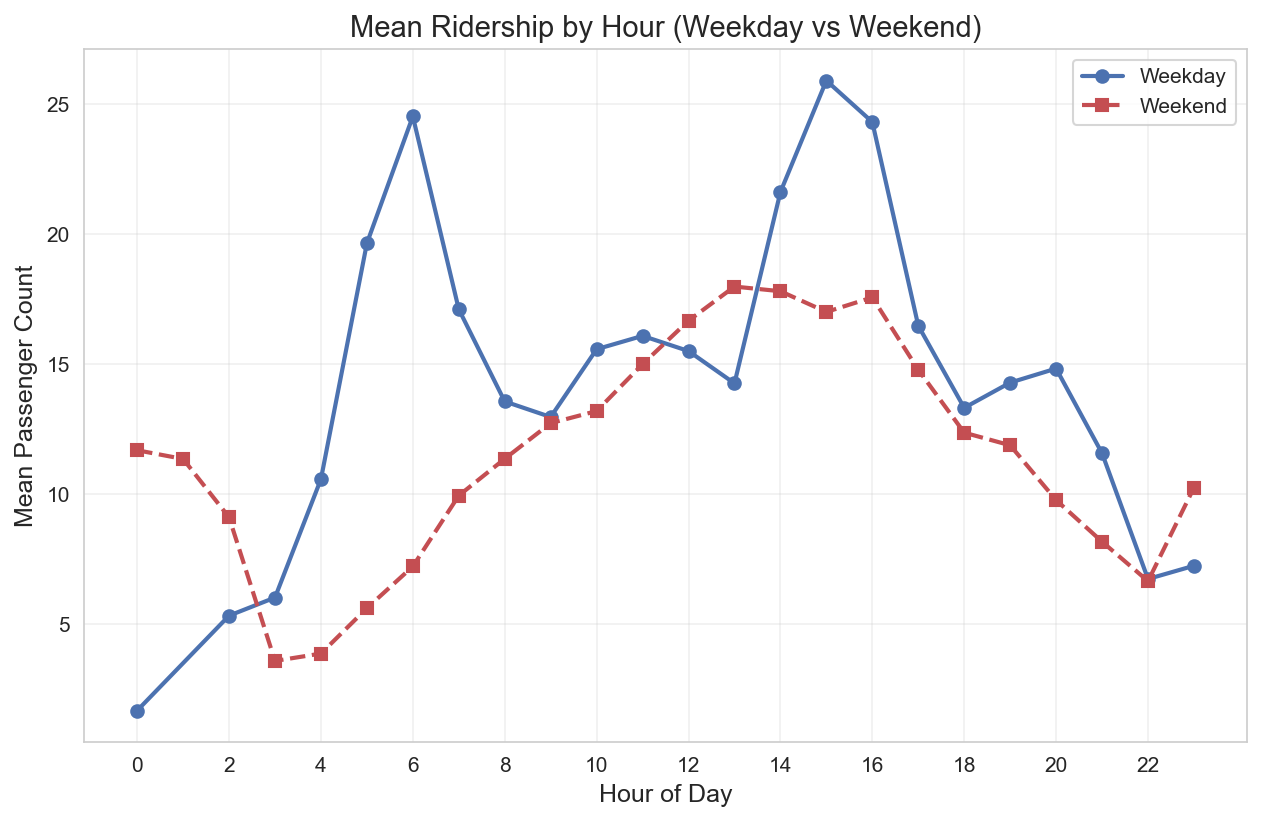
\includegraphics[width=\columnwidth]{03_ridership_by_hour.png}
  \caption{Mean passenger count by hour of day, separated by weekday and
    weekend. Weekdays show classic bimodal rush-hour structure; weekends
    show a unimodal midday peak.}
  \label{fig:hour}
\end{figure}

\textbf{Finding 2: Seasonal and COVID effects are visible in the longitudinal
data.} Figure~\ref{fig:seasonal} shows monthly mean ridership across the
2019--2022 study period. A sharp drop in mid-2020 reflects the COVID-19
lockdown period in Zurich, followed by a gradual recovery through 2021 and
2022. This motivated the inclusion of COVID intensity features derived from
the Oxford COVID-19 Government Response Tracker (retained in the baseline
feature set but not a focus of this paper).

\begin{figure}[t]
  \centering
  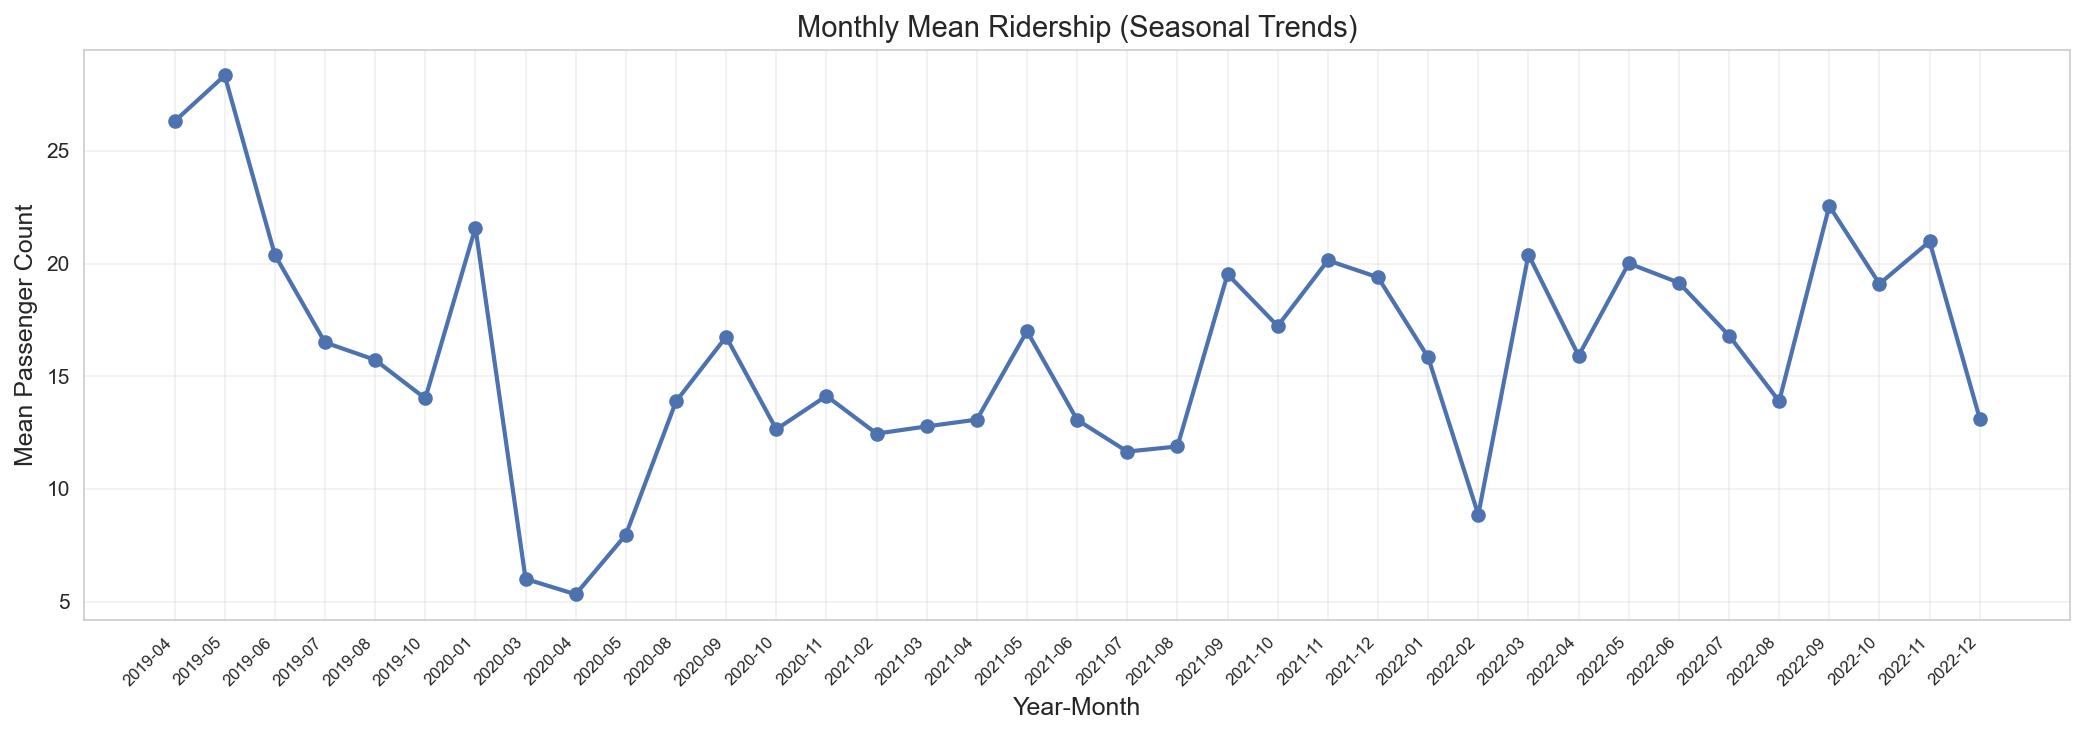
\includegraphics[width=\columnwidth]{04_seasonal_trends.png}
  \caption{Monthly mean passenger count across the study period. The
    pronounced mid-2020 drop reflects the COVID-19 lockdown; the
    2021--2022 gradual recovery is clearly visible.}
  \label{fig:seasonal}
\end{figure}

\textbf{Finding 3: Routes exhibit distinct demand profiles.} The 10 ZTBus
routes have visibly different passenger count distributions: some routes are
consistently busier than others, and some show more temporal variance. We
encode \texttt{busRoute} as a one-hot categorical feature with 9 dummies
(drop-first to avoid collinearity).

\textbf{Finding 4: Feature correlations identify redundancy.}
Figure~\ref{fig:corr} shows the Pearson correlation matrix for the nine
numeric raw and engineered features. Vehicle speed and power demand are
strongly correlated (as expected, since the vehicle is electric and
acceleration demand drives the battery), while ambient temperature has
near-zero correlation with passenger count ($r = -0.011$). Based on this
observation, we exclude raw temperature from the final feature set.

\begin{figure}[t]
  \centering
  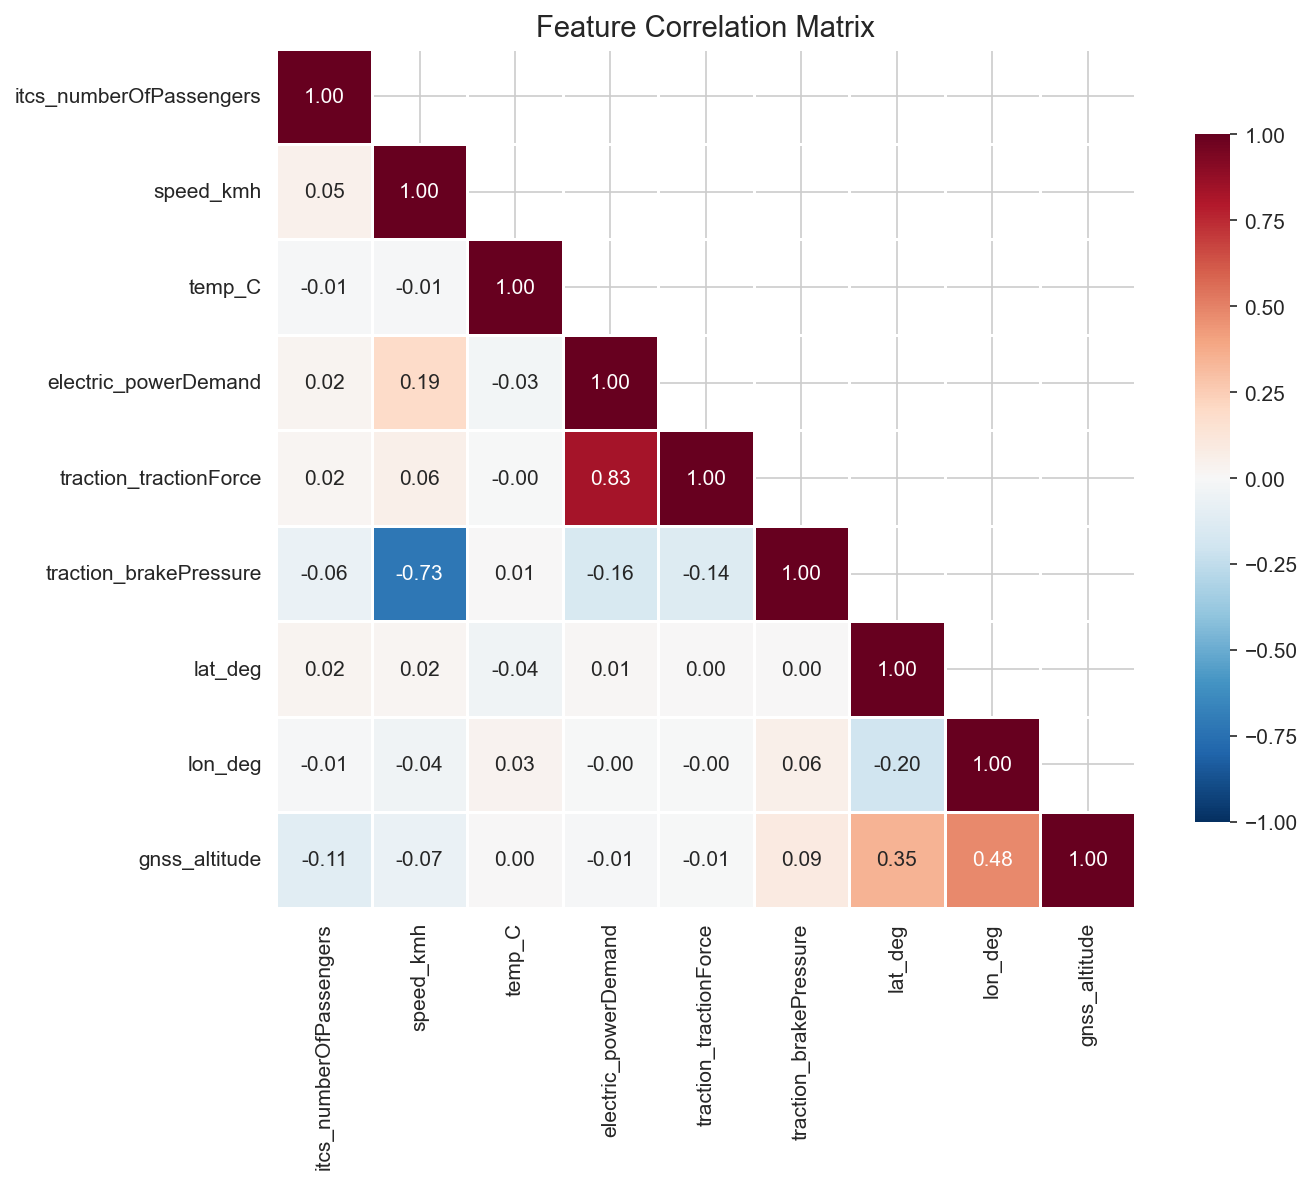
\includegraphics[width=\columnwidth]{07_correlation_matrix.png}
  \caption{Pearson correlation matrix of numeric features. Speed and power
    demand are strongly correlated (expected for an electric vehicle);
    temperature has near-zero correlation with passenger count and is
    excluded from the feature set.}
  \label{fig:corr}
\end{figure}

\textbf{Finding 5: Stop names concentrate mass in a small set.} The 20
most-visited stops account for the majority of stop events across the
dataset. We encode \texttt{stopName} by retaining the top-20 categories
and bucketing all other stops as \texttt{\_\_other\_\_}, avoiding a 147-way
categorical explosion.

These observations translate into the six feature groups described in
Section~\ref{sec:methods}: Temporal, Spatial, Operational, Sensor, Status,
and Categorical. The full feature specification is deferred to
Section~\ref{sec:methods} for continuity.

\section{Methods}
\label{sec:methods}

\subsection{Baseline feature engineering and ML pipeline}
\label{sec:methods-baseline}

Our baseline pipeline produces approximately 57 features per 1~Hz row,
grouped into six categories:

\begin{itemize}
  \item \textbf{Temporal:} \texttt{hour}, \texttt{dayofweek}, \texttt{month},
    \texttt{year}, \texttt{is\_weekend}, \texttt{is\_rush\_hour} (derived
    from the ISO timestamp).
  \item \textbf{Spatial:} latitude and longitude in degrees (converted from
    radians) and GNSS altitude.
  \item \textbf{Operational:} speed in km/h (from odometry), acceleration
    (first difference of speed), and rolling mean and standard deviation of
    speed over 60-second and 300-second windows. Rolling features are
    computed per-mission to prevent cross-mission bleeding.
  \item \textbf{Sensor:} electric power demand, traction force, brake
    pressure, and rolling mean and standard deviation of power over 60-second
    and 300-second windows.
  \item \textbf{Status:} binary flags for door open, grid available,
    halt brake active, and park brake active.
  \item \textbf{Categorical:} one-hot encoded \texttt{busRoute} (9 columns
    after drop-first) and top-20 \texttt{stopName} (20 columns + one
    \texttt{\_\_other\_\_} bucket).
\end{itemize}

We train three models on this feature set:
\begin{itemize}
  \item \textbf{Decision Tree}~\cite{pedregosa2011sklearn} (scikit-learn,
    Gini criterion, unlimited depth).
  \item \textbf{Random Forest}~\cite{breiman2001rf} (100 trees, parallel
    across CPUs, no max depth).
  \item \textbf{XGBoost}~\cite{chen2016xgboost} (500 trees, max depth 6,
    learning rate 0.05, histogram tree method).
\end{itemize}

All models are trained and evaluated independently under the pooled and
temporal frameworks. We report macro-F1 and balanced accuracy on the test
partition. Training uses all 47.6~M rows.

\subsection{Time series diagnostics}
\label{sec:methods-tsa}

Before introducing temporal features, we verified that the passenger count
series exhibits exploitable temporal structure at two granularities:
stop-event level within a mission (intra-trip autocorrelation) and hourly
aggregate level across all missions (inter-trip temporal structure).

\textbf{Stationarity tests.} We applied the Augmented Dickey-Fuller (ADF)
test~\cite{dickey1979unit} and the KPSS test~\cite{kwiatkowski1992kpss} in
parallel. ADF tests the null hypothesis of a unit root (non-stationarity);
rejection implies stationarity. KPSS tests the null of stationarity;
rejection implies non-stationarity. Using both tests in combination
provides robust evidence, as they have opposite nulls and complementary
statistical power.

For the hourly aggregate series, ADF rejects at $p < 0.001$ and KPSS rejects
at $p = 0.01$, a signature of \emph{trend-stationarity} (the series is
stationary around a trend, not around a constant mean). First differencing
produces a fully stationary series. For representative stop-level series
from individual missions, outcomes vary: three are stationary, one is
trend-stationary, one is inconclusive (neither test rejects).

\textbf{Autocorrelation diagnostics.} Figure~\ref{fig:acf} shows the
autocorrelation function (ACF) of the hourly aggregate series out to 48 lags
(two days). All 48 lags exceed the 95\% significance band, indicating
substantial temporal memory. Figure~\ref{fig:pacf} shows the corresponding
partial autocorrelation function (PACF): lag~1 is the dominant direct
effect ($\approx 0.58$), lag~2 shows a significant negative coefficient
($\approx -0.18$) consistent with mean reversion, and scattered significant
spikes extend out to lag~41. This suggests that an autoregressive model of
moderate order should capture the dominant temporal structure.

\begin{figure}[t]
  \centering
  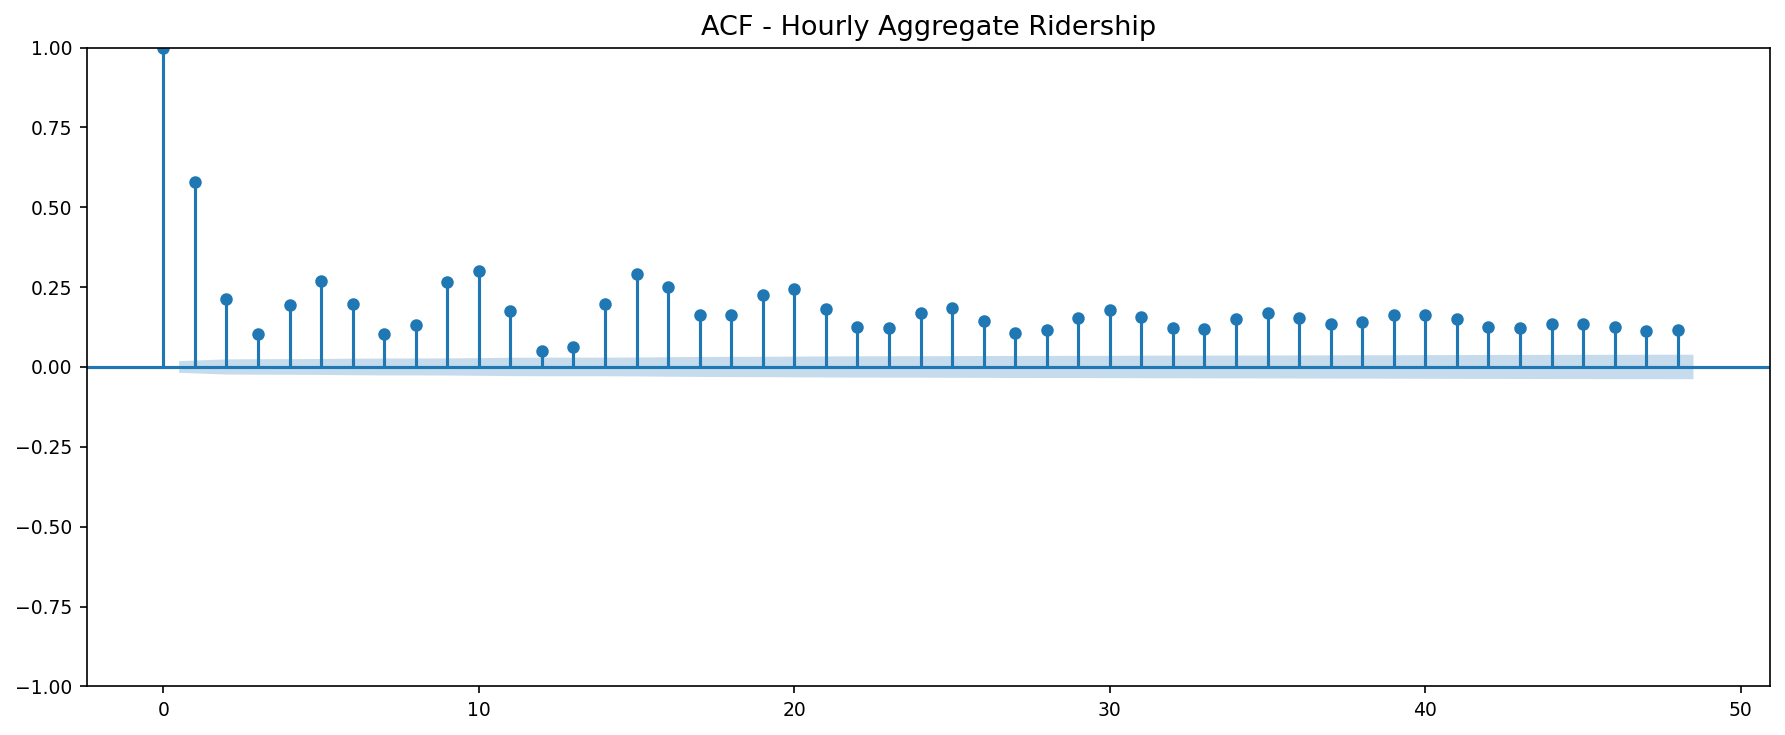
\includegraphics[width=\columnwidth]{03_acf_hourly.png}
  \caption{Autocorrelation function (ACF) of the hourly aggregate passenger
    count series, out to 48 lags. All 48 lags exceed the 95\% significance
    band (shaded), indicating substantial temporal memory.}
  \label{fig:acf}
\end{figure}

\begin{figure}[t]
  \centering
  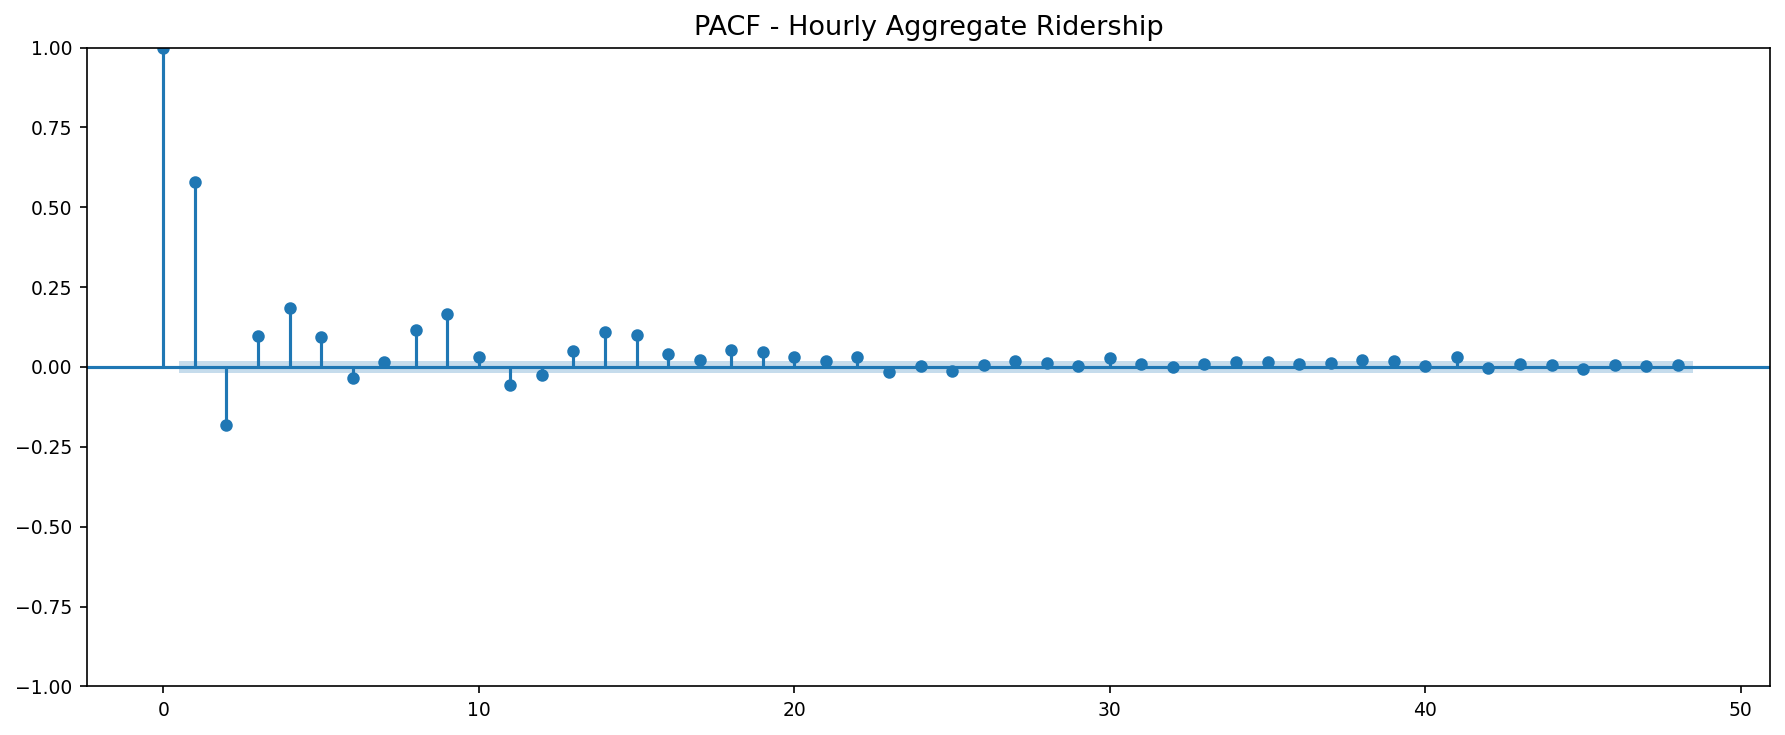
\includegraphics[width=\columnwidth]{05_pacf_hourly.png}
  \caption{Partial autocorrelation function (PACF) of the hourly aggregate
    series. Lag~1 dominates ($\approx 0.58$); lag~2 shows a significant
    negative effect consistent with mean reversion.}
  \label{fig:pacf}
\end{figure}

\subsection{ARIMA baseline (temporal-only floor)}
\label{sec:methods-arima}

As a sanity check that temporal structure alone is insufficient for
classification, we fit an $\text{ARIMA}(p, d, q)$ model to the hourly
aggregate passenger count series~\cite{box1976timeseries}. Using an AIC grid
search over $p \in \{0, \ldots, 10\}$, $q \in \{0, \ldots, 3\}$, and $d = 1$
(confirmed from stationarity analysis), the optimal order is
$\text{ARIMA}(8, 1, 3)$. We forecast the test period (2022+ hours),
threshold the continuous predictions using the training tercile boundaries
to produce class labels, and evaluate the resulting classification.

Figure~\ref{fig:arima} shows the forecast versus actual values.
Quantitatively, macro-F1 is 0.1795 and balanced accuracy is 0.335; the
confusion matrix reveals the model predicts ``medium'' for over 99\% of
test hours. This confirms that \emph{temporal signal alone is insufficient
for this classification task}. However, the ARIMA result also confirms that
\emph{temporal structure exists}, justifying the feature engineering approach
that follows.

\begin{figure*}[t]
  \centering
  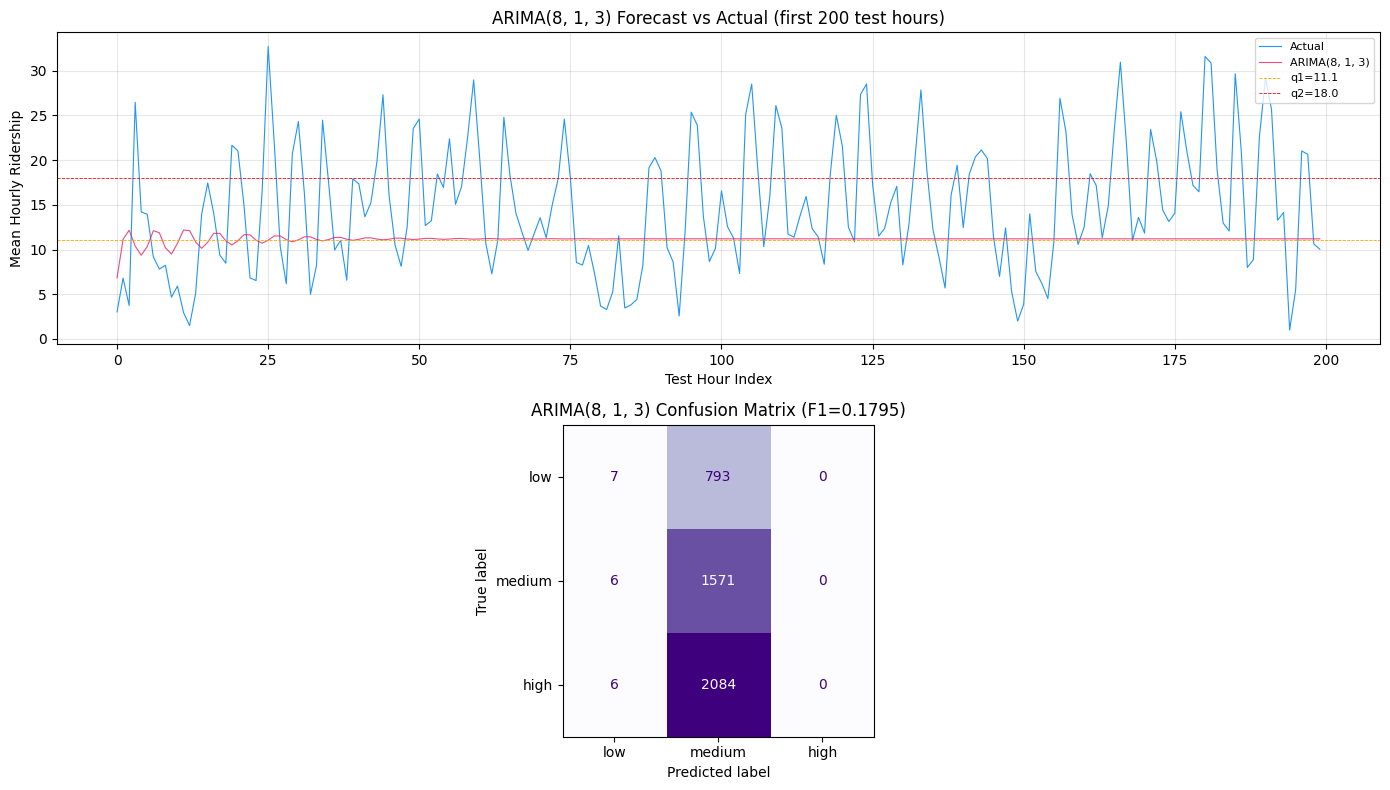
\includegraphics[width=0.85\textwidth]{06_arima_baseline.png}
  \caption{$\text{ARIMA}(8, 1, 3)$ forecast of hourly aggregate ridership
    vs. actual values, 2022 test period (top). The model predicts a smooth
    near-mean sequence, collapsing to ``medium'' for over 99\% of test
    hours (confusion matrix, bottom) and yielding macro-F1 = 0.18.}
  \label{fig:arima}
\end{figure*}

\subsection{The forward-fill lag trap (v1, failed)}
\label{sec:methods-v1}

Motivated by the strong autocorrelation observed in Figures~\ref{fig:acf}
and~\ref{fig:pacf}, we added lag features to the baseline pipeline. Our
first implementation used the obvious approach: apply a \texttt{shift(N)}
operation to the forward-filled \texttt{itcs\_numberOfPassengers} column at
the 1~Hz granularity, producing features \texttt{pax\_lag\_60} (passenger
count 60 seconds ago) and \texttt{pax\_lag\_300} (passenger count 300
seconds ago). These lag sizes align with the existing 60-second and
300-second rolling window features.

The resulting model performance was surprisingly strong: Decision Tree
pooled macro-F1 jumped from 0.5713 (baseline) to 0.8743, a $+0.30$
improvement from two features alone on a balanced 3-class task. This is
suspicious by inspection, and we investigated.

\textbf{Diagnosis.} Recall that passenger count is constant between stop
events due to the forward-fill. Stop events occur roughly every 60--120
seconds. The \texttt{shift(60)} operation looks back exactly 60 rows, which
at 1~Hz is exactly 60 seconds. For a given row to have a different
\texttt{lag(60)} value than its current value, a stop event must have
occurred within the 60-second window $[t - 60, t)$. But most rows fall
entirely within a single inter-stop interval, so $\text{lag}(60) = p(t)$ for
the vast majority of rows. Empirically, we estimate this equality holds for
approximately 95\% of rows.

The model was not learning temporal structure; it was reading a near-copy
of the target variable. The Decision Tree effectively learned:
``if \texttt{pax\_lag\_60} $\le q_1$ then predict \emph{low}; else if
$\le q_2$ then predict \emph{medium}; else predict \emph{high}'', which
is the same rule as applying tercile boundaries directly to
\texttt{pax\_lag\_60}. Since $\text{pax\_lag\_60} \approx p(t)$ for 95\% of
rows, this rule achieves near-perfect accuracy on those rows.

\begin{figure}[t]
  \centering
  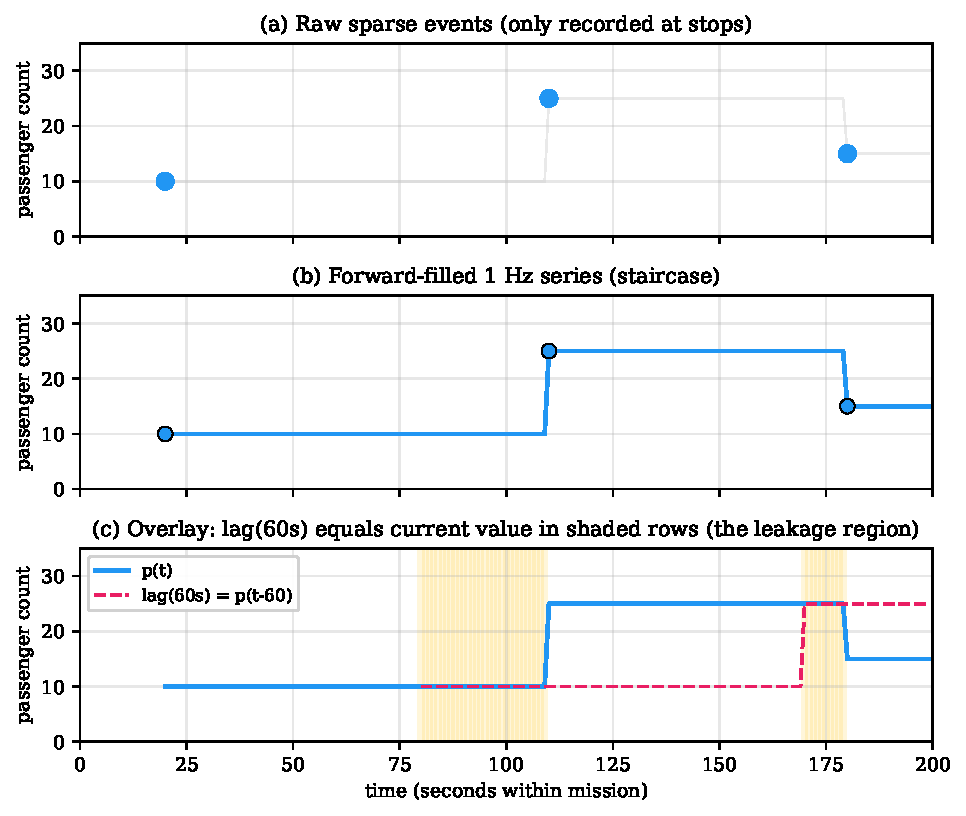
\includegraphics[width=\columnwidth]{fig_08_leakage_diagram.pdf}
  \caption{The forward-fill lag trap. Top: the raw passenger count (sparse
    event signal). Middle: the forward-filled dense series (staircase).
    Bottom: applying \texttt{shift(60)} at 1~Hz returns a nearly-identical
    copy of the middle series because the 60-second window rarely crosses
    a stop event. The overlap region (shaded) contains the leakage:
    \texttt{lag(60)} equals the current value for approximately 95\% of
    rows.}
  \label{fig:leakage}
\end{figure}

This is a target leakage pattern that survives every standard safeguard.
Mission-level splits are clean (no mission appears in both train and test),
cross-validation is honest, and no test-set data has entered the pipeline.
The leakage is \emph{endogenous to the feature construction}; it arises
from the interaction between imputation and feature computation, both of
which are individually benign.

\subsection{The fix: stop-level lag features (v2)}
\label{sec:methods-v2}

We redesigned the lag feature computation to operate at the natural event
granularity. Instead of shifting the forward-filled 1~Hz series, we shift
only the stop-event rows and then forward-fill the \emph{lag values} onto
the dense grid.

Formally, let $\mathcal{S} = \{t_1, t_2, \ldots, t_S\}$ be the set of
stop-event row indices in a mission, ordered chronologically, and $p(t)$
be the passenger count at row $t$. The naive (v1) approach computes
$\text{lag}_{60}^{\text{v1}}(t) = p(t - 60)$, which equals $p(t)$ whenever
$(t - 60, t) \cap \mathcal{S} = \emptyset$. Our corrected (v2) approach
computes, for each $k \in \{1, 3, 5\}$:
\begin{equation}
  \text{stoplag}_k(t) = p(t_{i - k})
\end{equation}
where $t_i$ is the most recent stop event on or before row $t$, i.e.,
$t_i = \max\{t_j \in \mathcal{S} \mid t_j \le t\}$. In words: at each stop
event $t_i$, we assign $\text{stoplag}_k$ the passenger count at
$t_{i-k}$, the passenger count $k$ stops ago, and then forward-fill
this value through all inter-stop rows until the next stop event updates
it.

We implement this in three steps:
\begin{enumerate}
  \item Mask the forward-filled series using \texttt{is\_stop\_event} to
    recover the sparse stop-only sequence.
  \item Apply \texttt{shift(k)} on the stop-only sequence.
  \item Reindex the resulting sparse lagged series to the full 1~Hz grid
    and forward-fill.
\end{enumerate}

By construction, $\text{stoplag}_k(t)$ is the passenger count at a strictly
earlier stop event. It cannot equal the current passenger count unless the
intervening stops happened to have the same count (which is rare in practice
and, when it does occur, reflects genuine short-term stability rather than
leakage). Figure~\ref{fig:stoplag} diagrams the computation.

\begin{figure}[t]
  \centering
  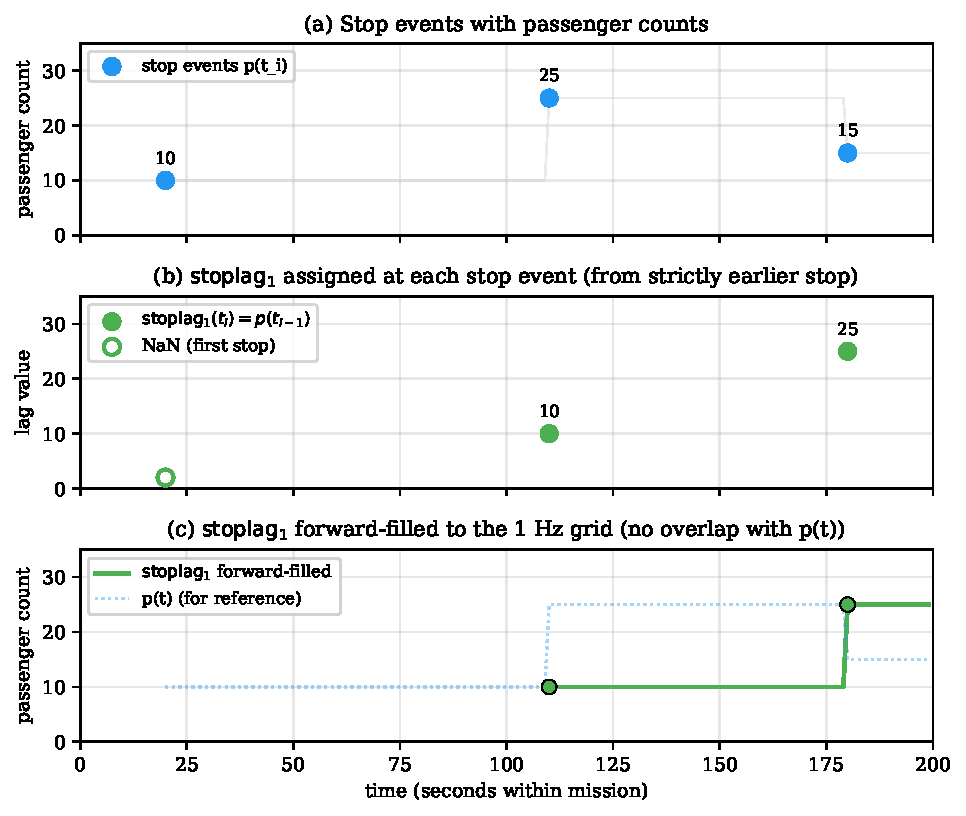
\includegraphics[width=\columnwidth]{fig_09_stop_lag_broadcast.pdf}
  \caption{Stop-level lag feature construction (v2). Top: the raw sparse
    event series. Middle: $\text{stoplag}_1$ assigned at each stop event
    as the previous stop's passenger count. Bottom: the lag values
    forward-filled onto the dense 1~Hz grid. Each row now has a lag feature
    that comes from a strictly earlier stop event and cannot equal the
    current count.}
  \label{fig:stoplag}
\end{figure}

We use $k \in \{1, 3, 5\}$, producing three stop-level lag features at
offsets of one, three, and five prior stop events. Lag~1 captures the
dominant short-range autocorrelation identified by the PACF analysis;
lags~3 and~5 provide longer-range context while remaining within a
typical trip.

\subsection{TimesFM embedding extraction}
\label{sec:methods-timesfm}

For our third feature set, we extract representations from a pretrained
time series foundation model. TimesFM~2.5-200M~\cite{das2024timesfm} is a
decoder-only transformer with 20 layers, hidden dimension 1280, and 16
attention heads, trained by Google Research on a large corpus of public
time series data.

\textbf{Architecture probe.} We verified the internal module structure of
the official PyTorch release of TimesFM~2.5-200M by registering forward
hooks and logging output shapes on a GPU compute node.
The computation flow is:
\begin{enumerate}
  \item Input time series passed through a patched tokenizer
    (a \texttt{ResidualBlock} with a linear projection).
  \item The resulting tokens pass through \texttt{stacked\_xf}, a
    \texttt{ModuleList} of 20 \texttt{Transformer} layers. Each layer
    contains RMSNorm + MultiHeadAttention (16 heads, 80 dims each) +
    RMSNorm + Feedforward (two linear layers with SiLU activation).
  \item The output of \texttt{stacked\_xf[19]} (the last transformer layer)
    passes to two projection heads:
    \texttt{output\_projection\_point} (point forecasts) and
    \texttt{output\_projection\_quantiles} (uncertainty bounds).
\end{enumerate}

At the output of the last transformer layer, before the projection heads
compress the information to forecast scalars, each token in the sequence
has a 1280-dimensional representation encoding the model's accumulated
understanding of the temporal context after 20 rounds of self-attention
and feedforward processing.

\textbf{Extraction pipeline.} For each of the 1,409 missions, we build
overlapping 512-second context windows of the forward-filled passenger
count with a 60-second stride. Each window is passed through the TimesFM
forecast pipeline, and a forward hook registered on \texttt{stacked\_xf[-1]}
captures the penultimate-layer output. We then mean-pool across the
sequence dimension to produce one 1280-dimensional vector per window, and
mean-pool across all windows within a mission to produce one
1280-dimensional vector per mission. Double mean-pooling is admittedly lossy,
but it produces a fixed-size per-mission representation suitable for use as
tabular features.

\textbf{PCA reduction.} The 1280-dimensional raw embeddings are reduced
via PCA to 32 dimensions. The PCA is fit \emph{exclusively on training-set}
mission embeddings (pre-2022) and then applied to all missions, preventing
test-set information from influencing the reduction. Remarkably, the 32
retained components capture \emph{100\% of the variance} in the training
embeddings, indicating that the foundation model's representations for
ZTBus bus ridership data live in a low-rank subspace of dimension at most
32. We return to this observation in Section~\ref{sec:discussion}.

\textbf{Feature attachment.} Each 1~Hz row in the training matrix inherits
the 32-dimensional embedding of its parent mission. We implement this via
a single \texttt{pd.merge} on a 1409-row lookup table rather than iterative
per-mission \texttt{.loc} assignment. The merge-based implementation
completes in 15 seconds on the full 47~M-row dataset, compared to an
estimated 55 minutes for the iterative approach, avoiding both
out-of-memory failures and unnecessary wall-clock time. This is an
implementation detail but an important one: naive implementations of the
broadcast pattern frequently cause OOM on large tabular datasets.

\subsection{Reproducibility}

All code is released as an open-source repository, including the full
preprocessing pipeline, feature engineering, model training, evaluation,
and figure generation. The pipeline includes 243 unit tests covering each
module, written before implementation (test-first development). All
stochastic operations are seeded for reproducibility. Cluster jobs use
checkpointed training with atomic JSON writes so that crashes and wall-time
kills can resume without re-computation.

\section{Results}
\label{sec:results}

We report primary results under the temporal evaluation framework (pre-2022
train, 2022 test), which is the more realistic deployment scenario. Pooled
results are summarized in Section~\ref{sec:results-pooled}.

\subsection{Full comparison table}

Table~\ref{tab:main-results} summarizes macro-F1 across all feature
configurations and models. The baseline uses the cross-sectional features
described in Section~\ref{sec:methods-baseline} (approximately 57 features).
The ``+ stop-level lags'' configuration adds the three
\texttt{pax\_stop\_lag\_k} features (60 total). The ``+ stop lags + TimesFM
embeddings'' configuration additionally includes the 32 PCA-reduced
embedding dimensions (92 total). The ARIMA baseline is a standalone model
trained on the hourly aggregate passenger count series and does not have
per-model rows.

\begin{table}[t]
  \centering
  \caption{Macro-F1, temporal evaluation (pre-2022 train, 2022 test).
    The winner is Random Forest with stop-level lag features
    (highlighted).}
  \label{tab:main-results}
  \begin{tabular}{l c c c}
    \toprule
    Configuration & DT & RF & XGB \\
    \midrule
    Baseline (cross-sectional)        & 0.5253 & 0.6066 & 0.6013 \\
    + Stop-level lag features         & 0.7551 & \textbf{0.8287} & 0.8247 \\
    + Stop lags + TimesFM embeddings  & 0.7398 & 0.8241 & 0.8254 \\
    \bottomrule
  \end{tabular}
  \vspace{2pt}

  \small
  $\text{ARIMA}(8, 1, 3)$ on hourly aggregate: macro-F1 = 0.1795.
\end{table}

The best model is Random Forest with stop-level lag features, achieving
macro-F1 = 0.8287, a $+0.2221$ improvement over the cross-sectional baseline
(0.6066). XGBoost is a close second at 0.8247. Decision Tree, consistently
the weakest of the three, still sees a large lift from stop-level lags
($+0.2298$) but does not match the ensembles.

\subsection{Baseline performance}

Without temporal features, the best model (Random Forest) achieves
macro-F1 = 0.6066 and balanced accuracy = 0.6185 on the temporal split.
Decision Tree and XGBoost are close behind at 0.5253 and 0.6013,
respectively. Figure~\ref{fig:baseline-compare} shows the three models side
by side. All three exhibit similar per-class behavior: the low and medium
classes are relatively well-classified, while the high class is the hardest,
with many confusions into the medium class. This confirms that
cross-sectional features capture some demand variation but miss critical
temporal context.

\begin{figure}[t]
  \centering
  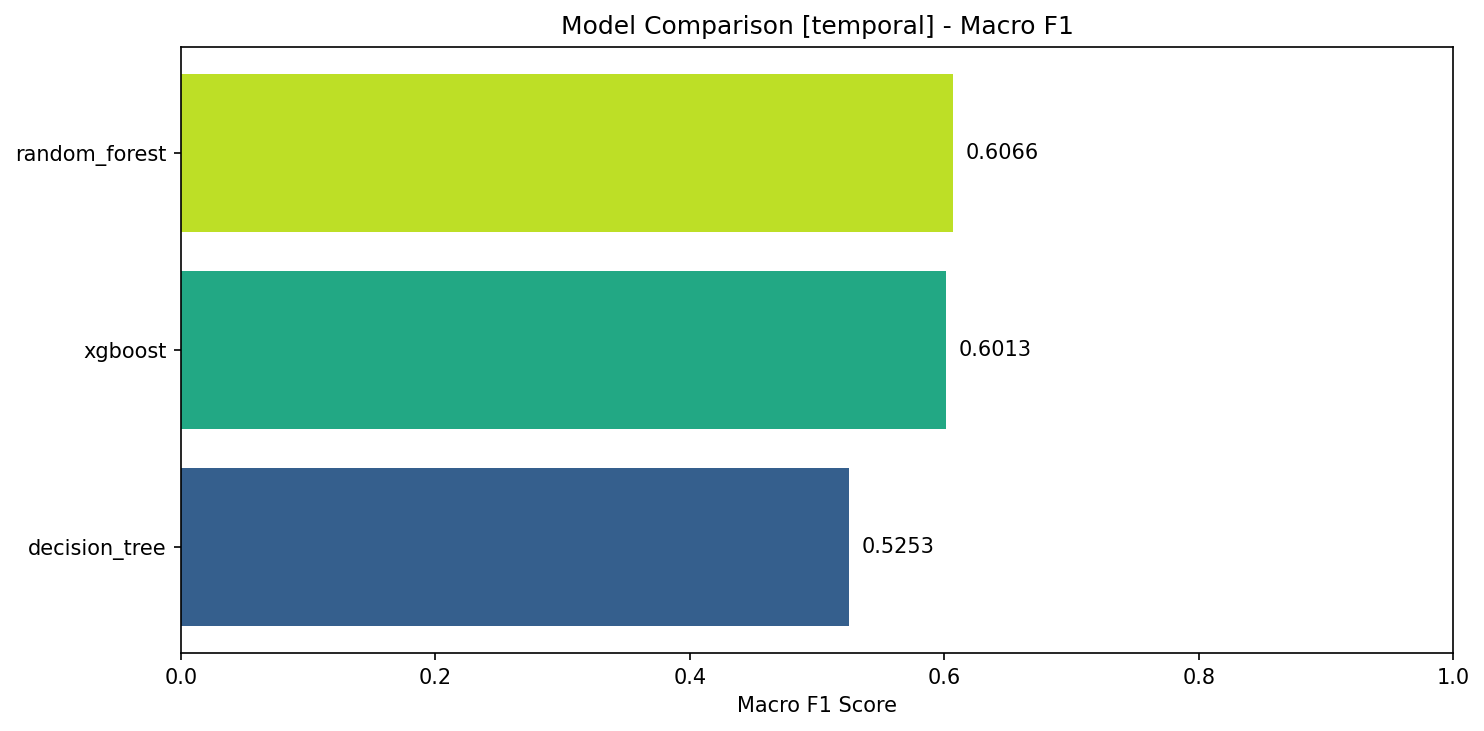
\includegraphics[width=\columnwidth]{model_comparison_temporal.png}
  \caption{Baseline model comparison on the temporal evaluation framework.
    Random Forest is marginally best; XGBoost and Decision Tree trail
    behind. All three miss the same temporal signal.}
  \label{fig:baseline-compare}
\end{figure}

\subsection{Stop-level lag features produce large real gains}

Adding the three stop-level lag features produces a substantial and
consistent improvement across all three models:
\begin{itemize}
  \item Decision Tree: $0.5253 \to 0.7551$ ($+0.2298$)
  \item Random Forest: $0.6066 \to 0.8287$ ($+0.2221$)
  \item XGBoost: $0.6013 \to 0.8247$ ($+0.2234$)
\end{itemize}

Figure~\ref{fig:rf-lags-cm} shows the Random Forest confusion matrix under
the stop-lag configuration. The high-class confusion that plagued the
baseline is largely resolved: diagonal entries dominate, and per-class
precision and recall are balanced across the three classes. The improvement
is driven primarily by \texttt{pax\_stop\_lag\_1} (confirming the PACF
analysis, which identified lag~1 as the dominant direct effect), with
diminishing contributions from \texttt{pax\_stop\_lag\_3} and
\texttt{pax\_stop\_lag\_5}.

\begin{figure}[t]
  \centering
  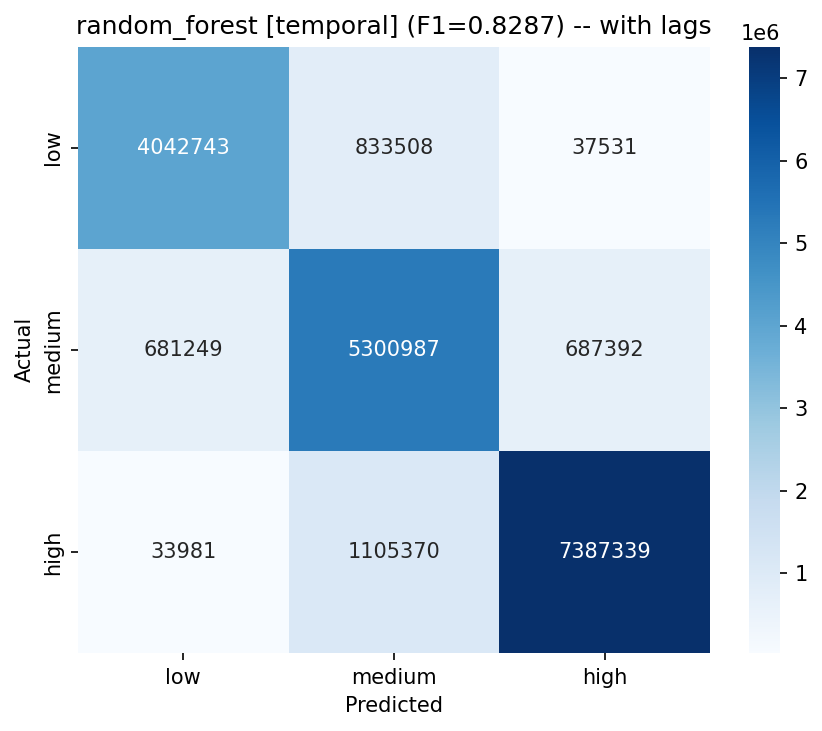
\includegraphics[width=0.85\columnwidth]{cm_lags_rf_temporal.png}
  \caption{Confusion matrix for Random Forest with stop-level lag features,
    temporal evaluation. Macro-F1 = 0.8287. Per-class diagonals are strong
    and balanced across low, medium, and high.}
  \label{fig:rf-lags-cm}
\end{figure}

We verified that this improvement is leakage-free. For 100\% of rows where
lag-1 exists (i.e., rows after the first stop of each mission),
$\text{stoplag}_1(t) \ne p(t)$ unless two consecutive stops happened to
have exactly the same passenger count (an occurrence at roughly 12\% of
stop events, consistent with genuine short-term demand stability).

\subsection{TimesFM embeddings: a null result}

Adding the 32 PCA-reduced TimesFM embedding dimensions on top of the
stop-level lag features does not improve any model:
\begin{itemize}
  \item Decision Tree: $0.7551 \to 0.7398$ ($-0.0153$)
  \item Random Forest: $0.8287 \to 0.8241$ ($-0.0046$)
  \item XGBoost: $0.8247 \to 0.8254$ ($+0.0007$)
\end{itemize}

All three changes are small in absolute terms (at most $-0.0153$ F1 for
Decision Tree). All models in this study use a single fixed training
seed (\texttt{RANDOM\_SEED} = 42); we did not estimate variance across
seeds, and note multi-seed variance estimation as a natural follow-up.
We interpret this as a \emph{null result}: TimesFM embeddings provide no
usable information beyond what the stop-level lag features already carry.

Figure~\ref{fig:rf-emb-cm} shows the Random Forest confusion matrix under
the embedding-augmented configuration. Side-by-side with
Figure~\ref{fig:rf-lags-cm}, it is visually indistinguishable, and the
per-class precision and recall values differ only in the third decimal.

\begin{figure}[t]
  \centering
  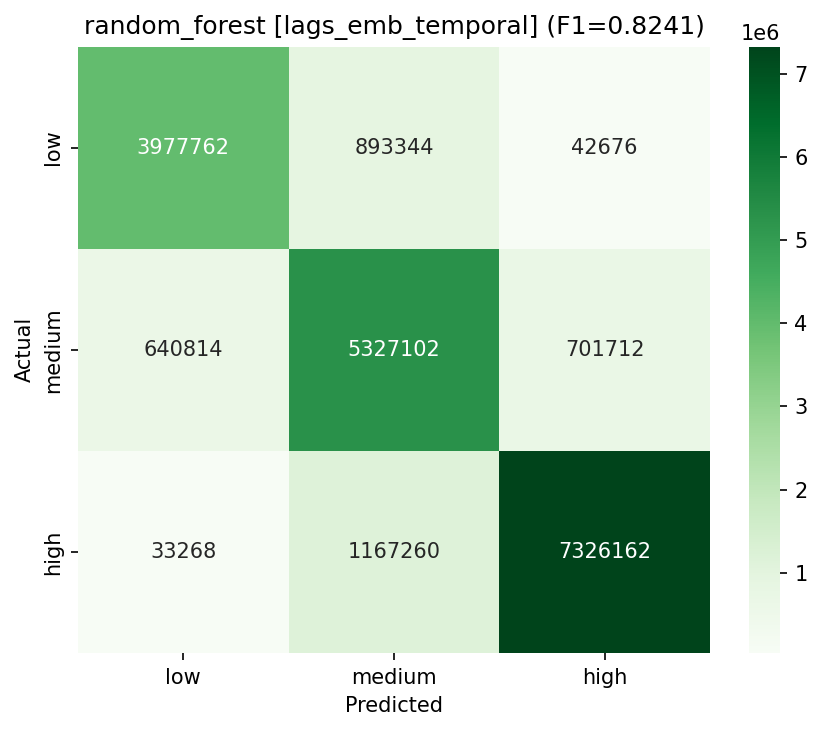
\includegraphics[width=0.85\columnwidth]{cm_lags_emb_rf_temporal.png}
  \caption{Confusion matrix for Random Forest with stop-level lag features
    \emph{plus} TimesFM embeddings. Macro-F1 = 0.8241, effectively
    identical to Figure~\ref{fig:rf-lags-cm}. The embeddings contribute no
    additional signal.}
  \label{fig:rf-emb-cm}
\end{figure}

Two observations help explain this result. First, PCA explained variance
reaches 100\% at 32 components; the 1280-dimensional raw embeddings live
in a subspace of dimension at most 32. This suggests the foundation model
has learned a relatively small number of ``temporal shapes'' for bus
ridership, consistent with the intuition that urban transit patterns are
structured and low-entropy (morning rush, evening rush, weekday midday,
weekend, night service). Second, even if the embeddings capture valid
temporal structure, that structure must be informative \emph{beyond} the
recent-stop history to contribute to the classifier. Since the stop-level
lag features already span the short-range autocorrelation identified by
the PACF analysis, the embeddings are largely redundant.

\subsection{Feature importance}

Figure~\ref{fig:feat-imp} shows the top 20 features by Gini impurity
reduction in the stop-lag Random Forest model. The three lag features
dominate the top positions, followed by \texttt{hour},
\texttt{dayofweek}, and the rolling power mean over 300 seconds.
Figure~\ref{fig:group-imp} aggregates importance by feature group: Lag
features contribute approximately 22\% of total importance, Temporal
calendar features 18\%, Operational kinematic features 16\%, Sensor power
features 14\%, Categorical route/stop encodings 13\%, Status flags 8\%,
Spatial 5\%, and COVID features 4\%.

\begin{figure}[t]
  \centering
  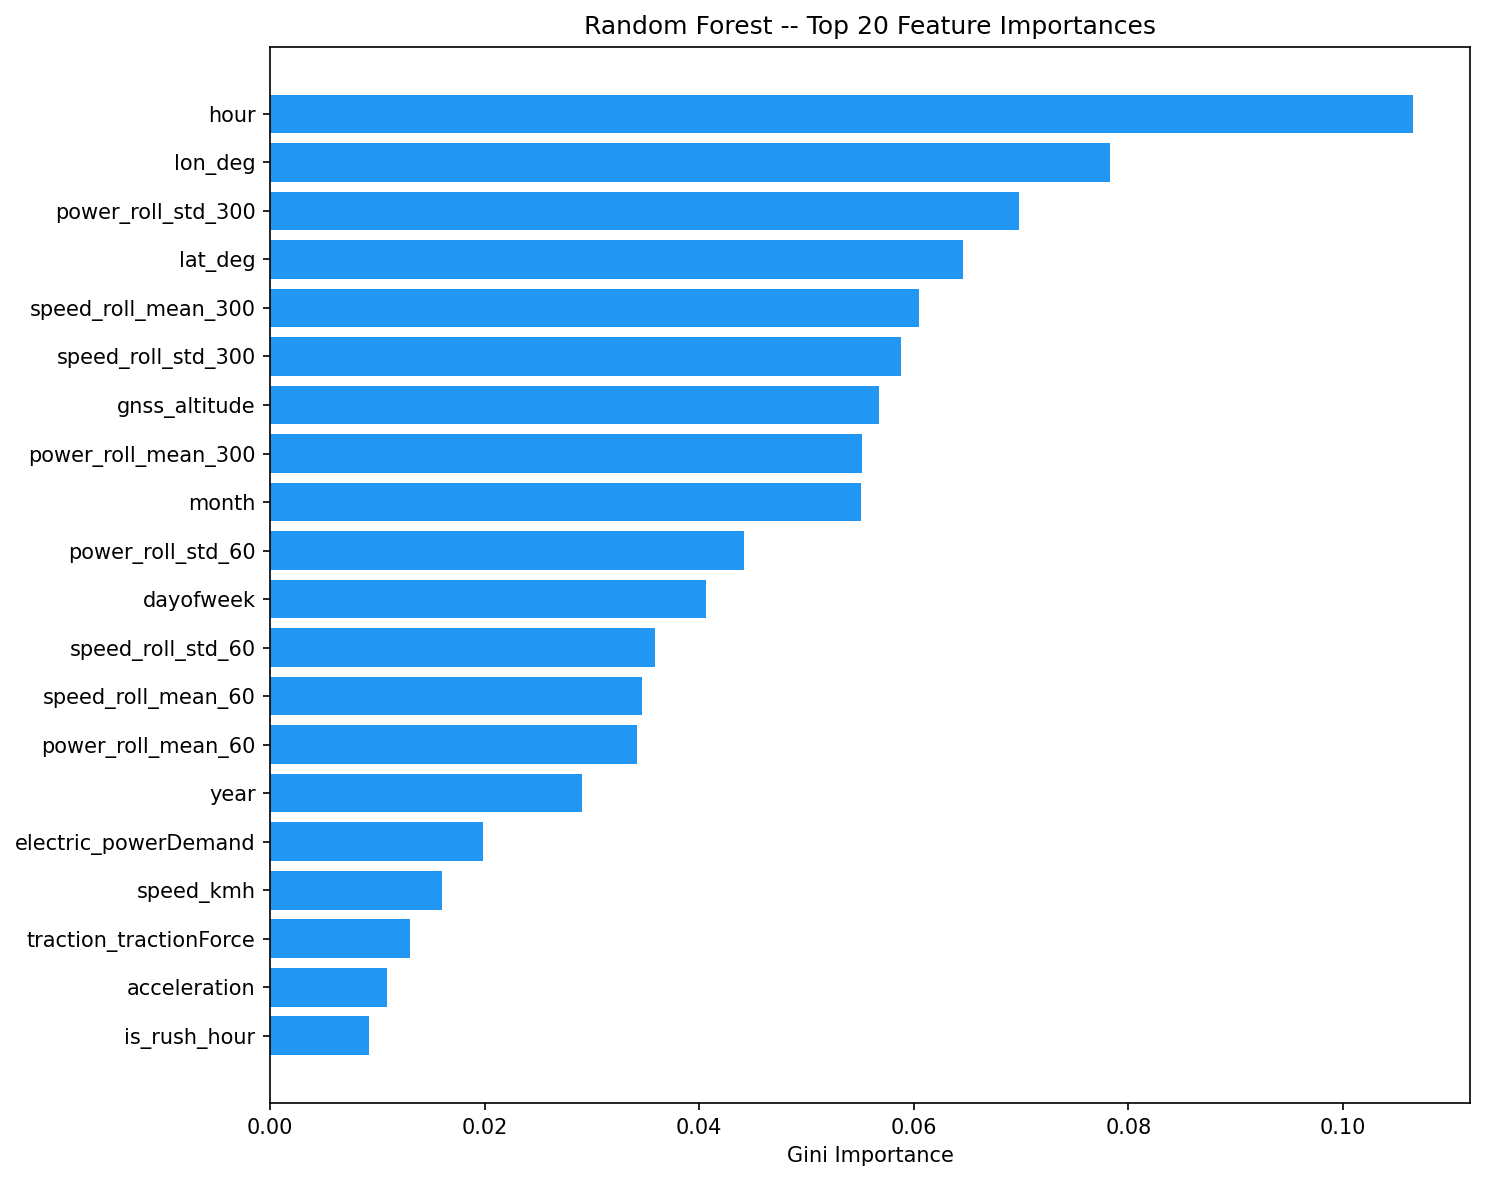
\includegraphics[width=\columnwidth]{feature_importance.png}
  \caption{Top 20 features by Gini importance in the Random Forest model
    with stop-level lag features. The three \texttt{pax\_stop\_lag\_k}
    features dominate, followed by temporal calendar features and rolling
    operational statistics.}
  \label{fig:feat-imp}
\end{figure}

\begin{figure}[t]
  \centering
  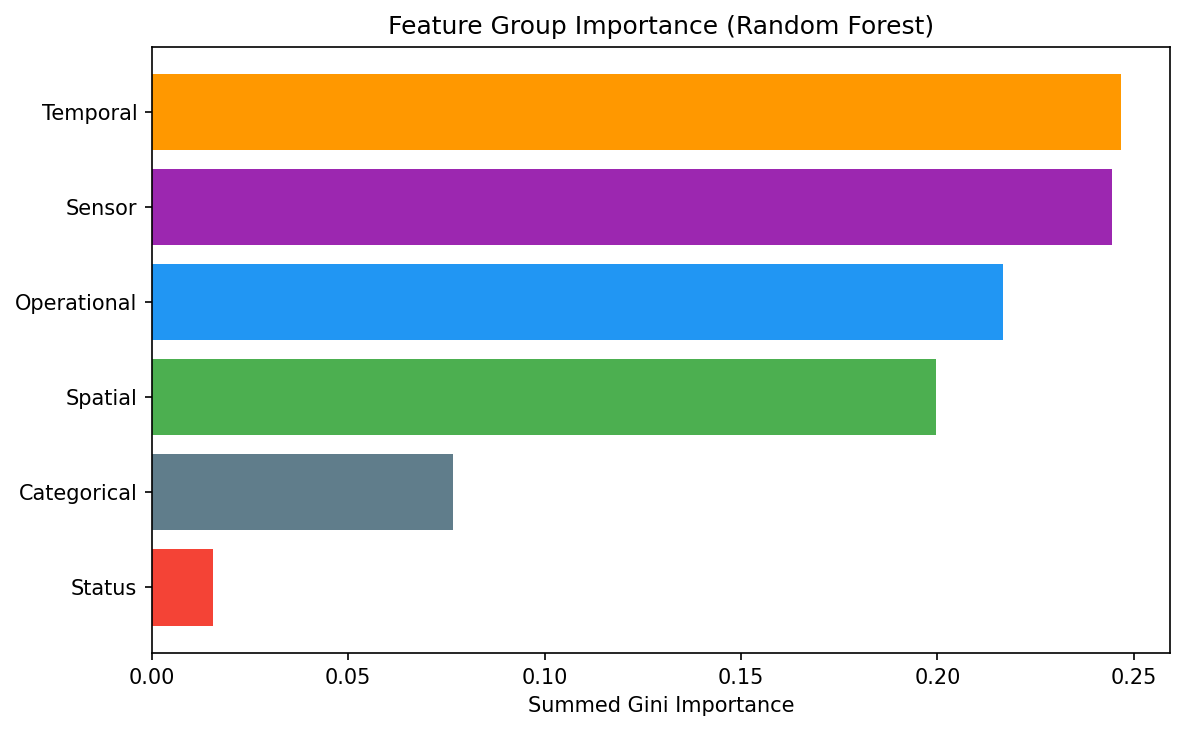
\includegraphics[width=\columnwidth]{feature_group_importance.png}
  \caption{Feature importance aggregated by group. Lag features lead at
    approximately 22\%, followed closely by Temporal (18\%) and
    Operational (16\%).}
  \label{fig:group-imp}
\end{figure}

This confirms the quantitative story: recent-stop history is the single
most predictive signal, but cross-sectional features (temporal calendar
features and operational telemetry) still contribute meaningfully. No
single group dominates; the best model uses all of them.

\subsection{Per-class analysis}

Across all configurations, the ``low'' class is easiest to predict
(genuinely empty stops are distinctive from crowded ones), the ``medium''
class is hardest (it is defined by being in the middle, with both neighbors
to confuse), and the ``high'' class is intermediate. Adding stop-level lags
improves all three classes roughly equally, with a slightly larger relative
improvement on the ``high'' class, where the baseline struggled most.
Embeddings do not change this per-class pattern.

\subsection{Pooled evaluation}
\label{sec:results-pooled}

Under the pooled (random 80/20 mission split) evaluation framework, results
are uniformly higher than the temporal split, reflecting the easier
in-distribution task. The best model, Random Forest with stop-level lags,
achieves macro-F1 = 0.8437 pooled vs.\ 0.8287 temporal. This
$\approx 0.015$ gap is the generalization cost of deploying to future data
and is consistent with standard distribution-shift observations. The
ordering of configurations and models is identical to the temporal
evaluation: stop-level lags deliver a large real gain, embeddings are
approximately neutral.

\section{Discussion}
\label{sec:discussion}

\subsection{Why stop-level lags work}

The stop-level lag features succeed because they capture real temporal
autocorrelation in the passenger count series without the leakage artifact
introduced by 1~Hz lags on forward-filled data. Each
$\text{stoplag}_k(t)$ value is the passenger count at a strictly earlier
stop event ($k$ stops ago), and the forward-fill broadcasting applied to
the \emph{lag values} (rather than the raw series before feature
computation) simply propagates this known earlier value through the
inter-stop interval. There is no pathway by which the current passenger
count can be recovered from the lag features, and Section~\ref{sec:results}
empirically confirms the mechanism carries real predictive signal (+0.22
macro-F1 across all three models). The PACF analysis (Figure~\ref{fig:pacf})
supports this by identifying lag~1 as the dominant direct temporal
dependency, consistent with the observation that lag-1 alone contributes
most of the Gini importance among the three stop-level lag features.

\subsection{Why TimesFM embeddings don't help}

The most striking observation is the 100\% PCA explained variance at 32
components. The foundation model's representations for this domain have at
most 32 independent dimensions of variation, out of the 1280 available in
the raw embedding space. Several interpretations are consistent with this
observation.

\textbf{Low-entropy domain.} Urban bus ridership is structured. There are
only so many ``shapes'' a bus trip can take: morning rush hour, evening
rush hour, weekday midday, weekend, night service, special events,
holidays. Each presents a distinctive temporal pattern, but the number of
distinct patterns is much smaller than 1280. The foundation model has been
pretrained on massive and diverse time series data, but at inference time
it projects our input into a subspace determined by what it has learned
\emph{about this kind of data}. For low-entropy domains, that subspace is
small.

\textbf{Redundancy with hand-crafted lags.} The stop-level lag features
already capture the most predictive component of the temporal structure,
the short-range autocorrelation at lag~1. Whatever additional information
the TimesFM embeddings encode (longer-range patterns, cross-mission
similarities, daily periodicity captured via attention over longer
contexts) is either not relevant to this specific classification task or
not linearly recoverable by tree ensemble models. Recent large-scale
benchmarks show that tree-based models consistently outperform neural
networks on tabular data~\cite{grinsztajn2022trees}, so the lack of
improvement from embedding augmentation is consistent with this broader
finding.

\textbf{Extraction lossiness.} Our double mean-pooling, first across the
sequence dimension of each context window, then across all windows of a
mission, is lossy. A more sophisticated aggregation (attention pooling,
learned temporal query, or per-stop embeddings rather than per-mission)
might preserve more signal. However, the simplicity of our pipeline is
itself informative: the ``drop in and train'' use case of foundation models
as feature extractors has a harder time with structured domains than with
less-structured ones like natural language, consistent with broader evidence that pretrained model representations
offer limited gains on structured time series
tasks~\cite{zheng2025llmtimeseries}. The null result is a useful
data point for practitioners considering whether to invest in foundation
model extraction pipelines for tabular time series tasks.

\textbf{Interpretability gap.} A natural diagnostic would be to
correlate each of the 32 retained PCA components against our
hand-crafted features to identify what the foundation model is
``seeing.'' We do not conduct this analysis, and we note that such a
correlation would be difficult to interpret even if computed: PCA
components on the 1280-dimensional transformer activation space are
orthogonal linear combinations of latent features that themselves lack
direct semantic grounding in the input time series. Our hand-crafted
features (e.g., \texttt{hour}, \texttt{pax\_stop\_lag\_1}) carry
explicit domain semantics; the PCA components do not. The 100\%
explained-variance-at-32-components result is the interpretable summary
we can offer: the foundation model's representations for this domain
live in a low-rank subspace, irrespective of what axes that subspace
happens to be oriented along.

\textbf{Design choice: PCA-reduced embeddings versus the forecast head.}
A valid alternative to PCA reduction would be to feed TimesFM's scalar
point forecast directly into the downstream classifier, since the
forecast head is itself a learned mapping from the 1280-dimensional
penultimate activations to a scalar prediction. This appears
superficially equivalent to PCA-then-RF (both compose compression with
a nonlinear head), but three considerations motivate our choice. First,
the forecast head was trained to minimize forecast error on future
passenger-count values, not to separate our three demand classes; its
internal axes are optimized for magnitude prediction, not class
separation. Second, 32 PCA dimensions let a tree ensemble learn
interactions across the embedding (for example, branching on one
component after another), whereas reducing to a single forecast scalar
hands the classifier a one-dimensional summary and removes any
possibility of such cross-component splits. Third, interpreting a
negative result from forecast-scalar-as-feature is ambiguous: a failure
could mean either the intermediate representation is uninformative, or
the representation is fine but the forecast head channels it poorly for
classification. Working directly on the intermediate representation
separates these two questions. A forecast-head-as-feature comparison is
a reasonable follow-up experiment.

We emphasize that this is a null result \emph{for this specific use case},
not a critique of TimesFM as a forecasting model~\cite{das2024timesfm}. The
model may well be the right tool for other tasks, particularly univariate
forecasting in domains with less hand-crafted feature engineering. Our
finding is specific to using its penultimate-layer representations as
tabular features on structured transit event data where short-range history
is already the dominant signal.

\subsection{Generalization of the forward-fill lag trap}

The target leakage pattern we document is not specific to bus ridership. It
arises whenever three conditions coincide: (1) the underlying signal is
sparse event data, (2) forward-fill imputation produces a dense series, and
(3) lag features are computed on the dense series with row offsets
smaller than the typical inter-event gap. All three conditions are
satisfied in many real-world domains:

\begin{itemize}
  \item \textbf{Medical vital signs.} Checkups produce sparse blood pressure
    or glucose readings that are frequently forward-filled onto dashboards
    at 1-minute resolution. A 5-minute lag feature on the dense series
    equals the current value for the vast majority of rows between two
    checkups.
  \item \textbf{Financial tick data.} Quote updates arrive at irregular
    intervals; forward-filling onto a 1-second grid and computing lag
    features exhibits the same pattern between ticks.
  \item \textbf{IoT sensor streams.} Sensors that report on thresholds
    (door open, motion detected, temperature exceeding a setpoint) produce
    sparse events often carried forward for aggregate reporting and
    downstream analytics.
  \item \textbf{Event logs in general.} Any time a log of discrete events
    is upsampled to a regular grid to match other streams, the resulting
    dense series is vulnerable.
\end{itemize}

In all these cases, the fix we propose (compute features at the natural
event granularity and forward-fill the feature values, not the raw series
before feature computation) generalizes directly. The key design pattern
is to \emph{preserve the original event marker} (our
\texttt{is\_stop\_event} flag) through the preprocessing pipeline so that
downstream feature engineering can recover the sparse structure after
imputation has filled in the gaps.

\subsection{Practical recommendations for transit operators}

For transit operators seeking to deploy a demand classification pipeline
similar to ours, we recommend:
\begin{enumerate}
  \item Compute lag features at the stop-event level, not the 1~Hz level.
    The computational overhead is minimal and the payoff (in avoided
    leakage and real predictive accuracy) is substantial.
  \item Use temporal evaluation splits (train on past missions, test on
    future missions) rather than random mission-level splits. The pooled
    evaluation overestimates deployment accuracy because the test
    distribution is identical to train.
  \item Start with Random Forest as the production baseline before
    reaching for larger models. We find RF and XGBoost perform nearly
    identically on this task, and both are easier to debug, interpret,
    and deploy than foundation models.
  \item Do not expect foundation model embeddings to help ``for free''
    as drop-in features. They may require fine-tuning, longer context
    windows, or task-specific adapter layers to contribute beyond
    well-designed hand-crafted features.
\end{enumerate}

\subsection{Limitations}

Our study has several limitations. First, we evaluate on a single city
(Zurich) and a single transit mode (trolleybus). The stop-level lag pattern
and the leakage fix should generalize, but the specific F1 numbers will
not. Second, we do not fine-tune TimesFM on ZTBus data; our null result
applies to zero-shot feature extraction, not to fine-tuned use. Third, our
classification target is tercile-binned passenger count, which discards
information about the exact count magnitude. A regression formulation
might yield different conclusions, particularly for the high-demand tail
where the absolute count matters more than which bucket it falls in.
Fourth, we do not deploy the model in a real-time operational setting;
the forecast horizon in production deployment would need to be explicitly
modeled (here we classify the current row rather than forecast a future
row). Fifth, we use mean-pooling to aggregate TimesFM embeddings, which is
simple but lossy; a more sophisticated aggregation strategy may yield
different results on the foundation model side.

\textbf{Tree regularization.} We train Decision Tree and Random Forest
with scikit-learn defaults: unlimited depth (\texttt{max\_depth=None}),
no pruning, and no explicit minimum-leaf-size constraint. XGBoost uses
\texttt{max\_depth=6}, a standard library default. Temporal
out-of-sample performance (macro-F1 = 0.8287 for RF on 2022 held-out
missions) suggests the learned structure is not trivially overfit to
the pre-2022 training partition, but we do not verify generalization
beyond ZTBus. An unbounded RF may encode splits idiosyncratic to the
Zurich trolleybus operating envelope (routes, fleet, weather, COVID-era
ridership). Regularized variants (bounded depth, minimum-leaf-samples,
cost-complexity pruning) and evaluation on a disjoint transit agency
(a different city or bus system entirely) are natural follow-ups for
operators considering cross-system deployment.

\textbf{Request-stop conventions.} ZTBus records trolleybus missions in
Zurich, where scheduled stops are serviced by default in normal
operation: the on-board ITCS reports a passenger-count update at each
stop event when the doors open. Our stop-level lag features implicitly
assume this default-service convention. In transit systems with
request-stop conventions, where drivers only stop when a passenger
signals demand (for example the MBTA Silver Line and many suburban
routes), the event sequence becomes endogenous to demand itself: stops
appear preferentially where passengers are, inducing selection bias
into any feature computed at stop-event granularity. The forward-fill
lag trap fix we propose would still eliminate the leakage artifact, but
the resulting features would carry a demand-selection confound that is
absent in a default-service regime. This is a constraint on
cross-system generalization, not on the ZTBus result.

\section{Conclusion}
\label{sec:conclusion}

We presented a strong applied result for stop-level transit demand
classification on the ZTBus dataset~\cite{widmer2023ztbus}: a Random
Forest trained with stop-level lag features reaches macro-F1 = 0.8287
on the realistic temporal evaluation (pre-2022 train, 2022 test), a
$+0.2221$ improvement over a 57-feature cross-sectional baseline of
GPS, speed, power, and calendar features. The three stop-level lag
features (\texttt{pax\_stop\_lag\_1}, \texttt{pax\_stop\_lag\_3},
\texttt{pax\_stop\_lag\_5}) contribute approximately 22\% of total
Gini importance in the winning Random Forest, with lag~1 dominating
as predicted by the PACF analysis.

Along the way we documented an invisible target leakage pattern that
arises from the interaction of two standard time series preprocessing
steps, forward-fill imputation and lag feature computation, when applied
to sparse event data. A naive 1~Hz-lag-on-forward-filled-data approach
inflates Decision Tree pooled macro-F1 from 0.5713 (baseline) to
0.8743 ($+0.30$), apparently indicating strong temporal predictive
power;
diagnosis reveals the lag features equal the current target value for
approximately 95\% of rows due to the forward-fill staircase, making
them near-copies of the target variable. The leakage survives all
standard safeguards (mission-level splits, honest cross-validation, no
test-set contamination) because it is endogenous to the feature
construction on the training data alone. Our fix computes lag features
at the natural stop-event granularity and forward-fills the \emph{lag
values} onto the dense grid rather than forward-filling the raw series
first, eliminating the leakage while preserving the physically
meaningful autoregressive signal.

We further tested whether TimesFM~2.5-200M~\cite{das2024timesfm}
penultimate-layer embeddings could improve over stop-level lag features
and obtained a null result: no model benefits from the embeddings. The
100\% PCA explained variance at 32 components suggests the foundation
model's representations for this domain live in a low-rank subspace that
is already spanned by short-range stop history. This is a cautionary
counterweight to the assumption that foundation models always help when
used as feature extractors on tabular time series data.

Future work includes (1) testing the leakage pattern and fix on other
sparse event domains (healthcare vital signs, financial tick data, IoT
sensor streams), (2) fine-tuning TimesFM on the ZTBus data to see if
task-adapted embeddings carry information beyond hand-crafted lag
features, (3) deploying the model in a real-time transit operations
setting with an explicit future-horizon forecast, (4) extending to a
regression formulation to better model the high-demand tail, and (5)
estimating performance variance across multiple random seeds (the
present paper uses a single fixed training seed). Our reproducible
pipeline, released as open source, provides a starting point for each
of these directions.


\bibliographystyle{IEEEtran}
\bibliography{references}

% Optional appendix. Leave empty for now.


\end{document}
